
\appendix

%%%%%%%%%%%%%%%%%%%%%%%%%%%%%%%%%%%%%%%%%%%%%%%%
% Apendice A
%%%%%%%%%%%%%%%%%%%%%%%%%%%%%%%%%%%%%%%%%%%%%%%%
\chapter{Edad escolar en diferentes Sistemas Educativos}\label{anexo:edad-educacion}

Incluso en la Unión Europea, los Sistemas Educativos difieren en la edad de escolarización de los estudiantes. Por ello, se ha confeccionado una tabla que intenta resumir la edad estándar en la que un niño está escolarizado durante las distintas etapas educativas\footnote{Se hablará de las etapas en las que el Sistema Educativo referido está bajo la responsabilidad del Ministerio de Educación (o equivalente) del propio país. Esto no excluye a la educación en centros privados.}. La información que se muestra a continuación está basado en \cite{cursos-educacion-europa} y \cite{guide-education-us}.

Se tomarán como referencia los nombres de las etapas del Sistema Educativo Español (Educación Infantil, Primaria, Secundaria y Bachillerato) para mostrar los años que pasan los estudiantes. Con respecto a la selección de países para realizar la comparación, se escogen los más representativos en los que se han realizado los estudios sobre el aprendizaje de la programación y donde más extendido están las plataformas que se mencionan en el presente documento. 


\begin{table}[!ht]
	\begin{centering}
		\begin{tabular}{c|c|c|c|c}
\emph{País} & Infantil & Primaria & Secundaria & Bachillerato\\
\hline
\emph{España} & 0-6 & 6-12 & 12-16 & 16-18\\
\emph{Estados Unidos} & 3-6 & 6-10 & 10-14 & 14-18\\
\emph{Reino Unido} & 2-5 & 5-11 & 11-16 & 16-18\\
\emph{Alemania} & 0-6 & 6-10 & 10-16 & 16-19\\
\emph{Francia} & 2-6 & 6-11 & 11-16 & 16-18\\
\emph{Bélgica} & 0-2.5/3 & 2.5/3-6 & 6-12 & 12-18\\
\emph{Irlanda} & 4-6 & 6-12 & 12-15 & 15-19\\
\end{tabular}
	\caption{Comparativa de edades de escolarización en diferentes Sistemas Educativos con respecto a las etapas del Sistema Educativo Español.}
		\label{tab:comparativa-tecnicas}
	\end{centering}
\end{table}

En el caso del Sistema Educativo Americano, existen muchas vías en la formación de un niño, como bien detalla A. Corsi-Bunker en \cite{guide-education-us}. Dependiendo de si se escoge una vía privada o dependiendo del estado, los años pueden variar. Aún así, en la figura \ref{tab:comparativa-tecnicas} se muestra el modelo estándar (sistema K-12).\footnote{Para más información sobre el Sistema Educativo Americano recomiendo que se acuda directamente a la fuente: U.S. Department of Education, National Center for Education Statistics (\url{http://nces.ed.gov})}.

\begin{figure}[!ht]
	\begin{centering}
		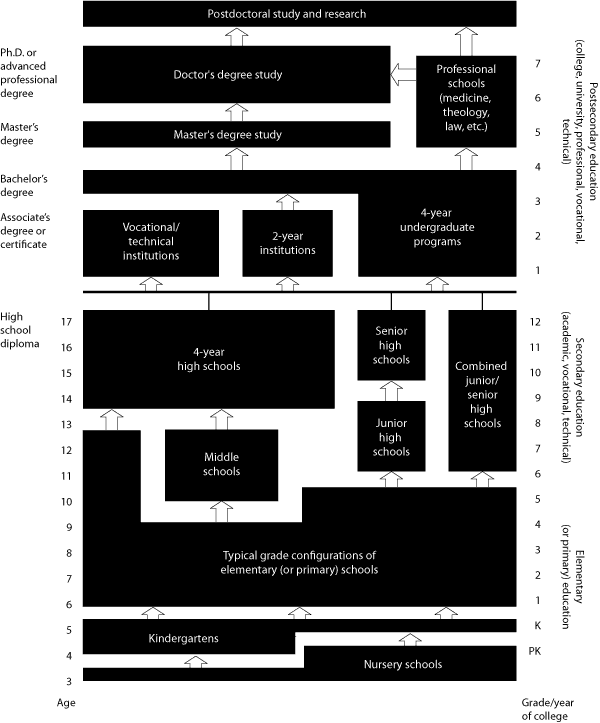
\includegraphics[width=0.75\textwidth]{images/education-usa.png}
			\caption{Tabla que muestra los típicos patrones de progresión en el Sistema Educativo Americano. Fuente: U.S. Department of Education, National Center for Education Statistics, Annual Reports Program. Obtenido de \url{http://nces.ed.gov/programs/digest/d11/figures/fig_01.asp}}
				\label{fig:education-usa}
	\end{centering}
\end{figure}





%%%%%%%%%%%%%%%%%%%%%%%%%%%%%%%%%%%%%%%%%%%%%%%%
% Apendice B
%%%%%%%%%%%%%%%%%%%%%%%%%%%%%%%%%%%%%%%%%%%%%%%%
\chapter{Lenguaje Logo}
\label{anexo:logo-lenguaje}

A continuación se realizará una revisión de las principales características del lenguaje Logo para tener una visión general de su funcionamiento y sintaxis. Este análisis se basa en el trabajo de \cite[p.274-305]{feurzeig1969programming}. Si el lector quiere ampliar información sobre el lenguaje Logo, puede consultar \cite{friendly2014advanced} o \cite{logo-resources}.


\section{\emph{words}, \emph{sentences}, operaciones y comandos}

Hay dos tipos de datos principales: \emph{words} y \emph{sentences}. \emph{words} está formado por 0 o más caracteres, sin espacios. Algunos ejemplos son: "SUN", "CAT", "5",  "97&!", "" (cadena vacía). El tipo de datos \emph{sentences} se forma por un conjunto de \emph{words} separado por espacios, como por ejemplo "HELLO WORLD" o "3 + 2 = 5". Un numero es una \emph{word} pero conpuesto únicamente por dígitos.

En el lenguaje Logo existen operadores para tratar con los tipos \emph{words} y \emph{sentences}. También se pueden encontrar una serie de operaciones predefinidas en el lenguaje que ofrecen funcionalidad extra, como controlar la entrada/salida de un programa, saber la fecha o manejo de \emph{words} y \emph{sentences}. En la tabla \ref{tab:logo-operaciones} vemos un resumen de las operaciones elementales del lenguaje Logo, el número de argumentos que requiere y un ejemplo de entrada con su salida correspondiente.


\begin{table}[!ht]
	\begin{centering}
		\begin{tabular}{c|c|c|c}
\emph{Operador} & N. argumentos & Entrada & Salida\\
\hline
\texttt{FIRST}	& 1 & "CAT" & "C"\\
- & - & "CAT AND DOG" & "CAT"\\
\texttt{LAST} & 1 & "CAT" & "T"\\
- & - & "CAT AND DOG" & "DOG"\\
\texttt{BUTFIRST} &1& "CAT" & "AT"\\
- & - & "CAT AND DOG" & "AND DOG"\\
\texttt{BUTLAST} & 1 & "CAT" & "CA"\\
- & - & "CAT AND DOG" & "CAT AND"\\
\texttt{COUNT} & 1 & "CAT" & "3"\\
- & - & "CAT DOG" & "2"\\
\texttt{WORD}& 2 & "CAT" "DOG" & "CATDOG"\\
\texttt{SENTENCE}& 2 & "CAT" "DOG" & "CAT DOG"\\
- & - & "CAT " "DOG" & "CAT DOG"\\
\texttt{PRINT} & 1 & "CAT" & CAT\\
\texttt{TIME} & 0 & - & "5:42 PM"\\
\texttt{DATE} & 0 & - & "1/31/2016"\\
\texttt{SUM} & 2 & "-5" "5" & "0"\\
\texttt{DIFFERENCE} & 2 & "5" "5"& "0"\\
\texttt{MAXIMUN} & 2 & "-5" "5" & "5"\\
\texttt{MINIMUN} & 2 & "3" "5"& "3"\\
\end{tabular}
	\caption{Resumen de las operaciones elementales que ofrece el lenguaje Logo.}
		\label{tab:logo-operaciones}
	\end{centering}
\end{table}

Si se intentara ejecutar la operación \texttt{WORD} "CAT " "DOG", se produciría un error al ser uno de sus parámetros un tipo \emph{sentence} y no \emph{word} (el primer argumento contiene un espacio). De igual manera, las operaciones \texttt{SUM}, \texttt{DIFFERENCE}, \texttt{MAXIMUN} y \texttt{MINIMUN} deben recibir argumentos numéricos o se produciría un error.

También es posible encadenar varios operadores. De esta manera, la cadena de instrucciones \texttt{FIRST OF BUTFIRST OF "CAT"} devolverá el \emph{word} "A".


\section{Variables, comentarios y definiendo nuevas operaciones}
\label{sec:logo-variables}

Para definir variables basta con usar el operador \texttt{MAKE} seguido de \emph{"}(comilla doble), el nombre de la variable y el valor que se quiere asignar. Para hacer uso de la variable, utilizamos el símbolo \emph{:}(dos puntos) seguido del nombre de la variable. Para hacer comentarios se utiliza el símbolo \emph{;}(punto y coma). Podemos ver un ejemplo en el código \ref{code:logo-nueva-variable}.

\begin{lstlisting}[language={Logo}, label={code:logo-nueva-variable}, caption={Ejemplo de definición de nuevas variables en el lenguaje Logo.}]
MAKE "ADULTO 18

PRINT :ADULTO  ; salida -> 18
\end{lstlisting}

También es posible crear nuevas operaciones. Se utilizan las palabras reservadas \texttt{TO} y \texttt{END} para marcar el inicio y final de la definición, respectivamente. A continuación es necesario declarar el nombre con el que se definirá la operación que se está creando (el cual no puede coincidir con ninguna palabra reservada en el lenguaje, como es común en la mayoría de lenguajes de programación). Es opcional la declaración de parámetros que se pasaran a la operación. Por último, y antes de la palabra \texttt{END}, se incluirán las instrucciones que realizará la operación.

En el código \ref{code:logo-nuevas-operaciones} se puede ver un ejemplo de definición de nuevas operación.

\begin{lstlisting}[language={Logo}, label={code:logo-nuevas-operaciones}, caption={Definición de nuevas operaciones en el lenguaje Logo.}]
TO SALUDAR
	MAKE "SALUDO "HELLO WORLD"
	OUTPUT SALUDO
END

PRINT SALUDAR  ;  salida -> HELLO WORLD

TO PENULTIMO :algo
	OUTPUT FIRST OF  LAST :algo
END

PRINT PENULTIMO OF "CAT BIRD DOG" ;  salida  ->  BIRD

PRINT PENULTIMO OF "CAT" ;  salida  ->  A
\end{lstlisting}


\section{Operadores aritméticos}

A parte de los operadores \texttt{SUM} y \texttt{DIFFERENCE} antes mencionados, Logo también otorga la posibilidad de utilizar los operadores aritméticos clásicos. La única condición es que la salida generada debe ser tratada (\texttt{PRINT}) o almacenada (en variables, como veremos en la sección siguiente) de alguna manera. Los operadores más importantes son \texttt{+}, \texttt{-}, \texttt{*}, \texttt{/} y \texttt{sqrt}.

\begin{lstlisting}[language={Logo}, label={code:logo-operadores-aritmeticos}, caption=Ejemplo de uso de operadores aritméticos en el lenguaje Logo.]
PRINT 2*3  ;  salida  -> 6

MAKE "RUEDAS  4

PRINT :RUEDAS ;  salida  -> 4
\end{lstlisting}


\section{Operadores \texttt{IF} y \texttt{REPEAT}}

Se pueden crear operaciones condicionales utilizando la palabra clave \texttt{IF} seguida de una sentencia y una lista de órdenes a ejecutar si se evalúa dicha sentencia a verdadero. La lista de órdenes se declara entre corchetes (\texttt{[]}) y para la sentencia se pueden utilizar los operadores infijos \texttt{=}, \texttt{>} y \texttt{<}. En el código \ref{code:logo-if} podemos ver un ejemplo de uso.

\begin{lstlisting}[language=Logo,label={code:logo-if}, caption=Condiciones en el lenguaje logo con el operador \texttt{IF}.]
MAKE "PETALOS 4

IF :PETALOS > 3 [ PRINT "TREBOL DE LA BUENA SUERTE" ]
\end{lstlisting}

Para repetir una serie de instrucciones, Logo ofrece el comando \texttt{REPEAT}, que va seguido de un valor numérico y la lista de instrucciones. El valor numérico (que puede ser parametrizado) es el número de veces que se repetirá en bucle las instrucciones. En el código \ref{code:logo-repeat} vemos un ejemplo de este comando.


\begin{lstlisting}[language=Logo,label={code:logo-repeat}, caption=Condiciones en el lenguaje logo con el operador \texttt{IF}.]
REPEAT 10 [ PRINT "HOLA MUNDO" ]
\end{lstlisting}



